\subsection{Approach}
\label{sec:soft_cut_approach}

For the soft cut detection we decided to use a deep learning approach.
More concrete we used the RNN/LSTM implementation by Jeff Donahue\footnote{\url{https://github.com/BVLC/caffe/pull/2033}}. \\
This RNN/LSTM implementation takes two different inputs: On the one hand the raw pixel values and on the other hand a tagging sequence.
A tagging sequence represents sequences of frames, where one sequence of frames might represent a soft cut in our case.
Using this implementation allows us to incorporate the information of a frame, which is at the beginning of a frame sequence, to a frame, which is located later in the same sequence.
So the net memorizes previous decision along a sequence of frames. \\
But using this architecture has one problem, as stated by Jeff Donahue: ``Backpropagation [through the LSTM] is truncated along the batch boundaries'' [TODO: Quelle].
So one or more frame sequences has to fit exactly into the batch size used by the RNN/LSTM.
This is hard to archive if we want to use variable length of frame sequences.
Therefore we decided to use a fixed size for the sequences of frames in a tagging sequence, i.e. we only check for example ten consecutive frames of being a soft cut or not.  \\
However, we still want to find soft cut of arbitrary length in a video.
To achieve this, we repeatedly test fixed-size frame sequences.
In Figure~\ref{fig:soft_cut_approach} an example is shown.
\begin{figure}[!htb]
	\centering
	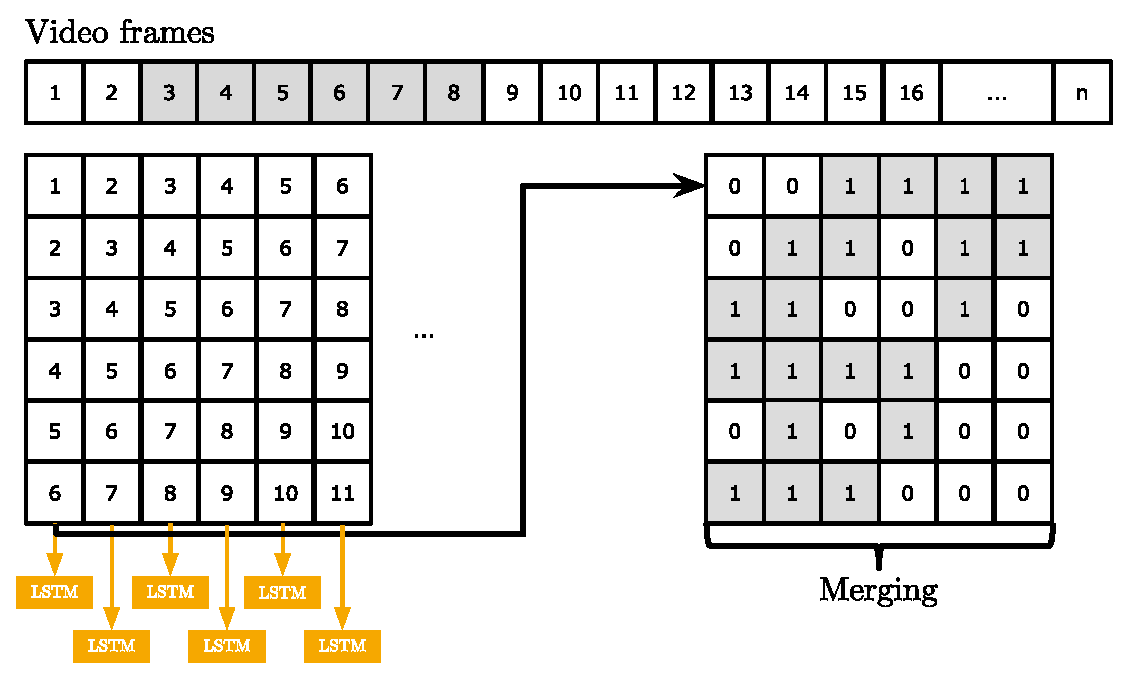
\includegraphics[scale=.7]{images/soft_cut_approach.eps}
	\caption{To classify soft cuts of arbitrary length, we repeatedly test fixed-size frame sequences. In this example we test sequences of size six. Afterwards the predictions given by the RNN/LSTM are merged, so that we have one prediction per frame.}
	\label{fig:soft_cut_approach}
\end{figure}
We have a video with \textit{n} frames.
The frames from three to eight represent a soft cut.
We now generated for each frame a frame sequence of size six.
Those sequences are then classified by the RNN/LSTM.
The output of the RNN/LSTM is zero, if a frame does not belong to a soft cut, and one, otherwise.
In the end we have up six prediction per frame, which have to be merged, so that we only have one prediction per frame.
After the merging step consecutive frames, which got a prediction of one, i.e. the frame is part of an soft cut, represent a soft cut. \\
In the following several strategies for combining the multiple frame prediction into one prediction are presented.
An overview over all strategies can be found in Figure~\ref{fig:merging_strategies}.
\begin{figure}[!htb]
	\centering
	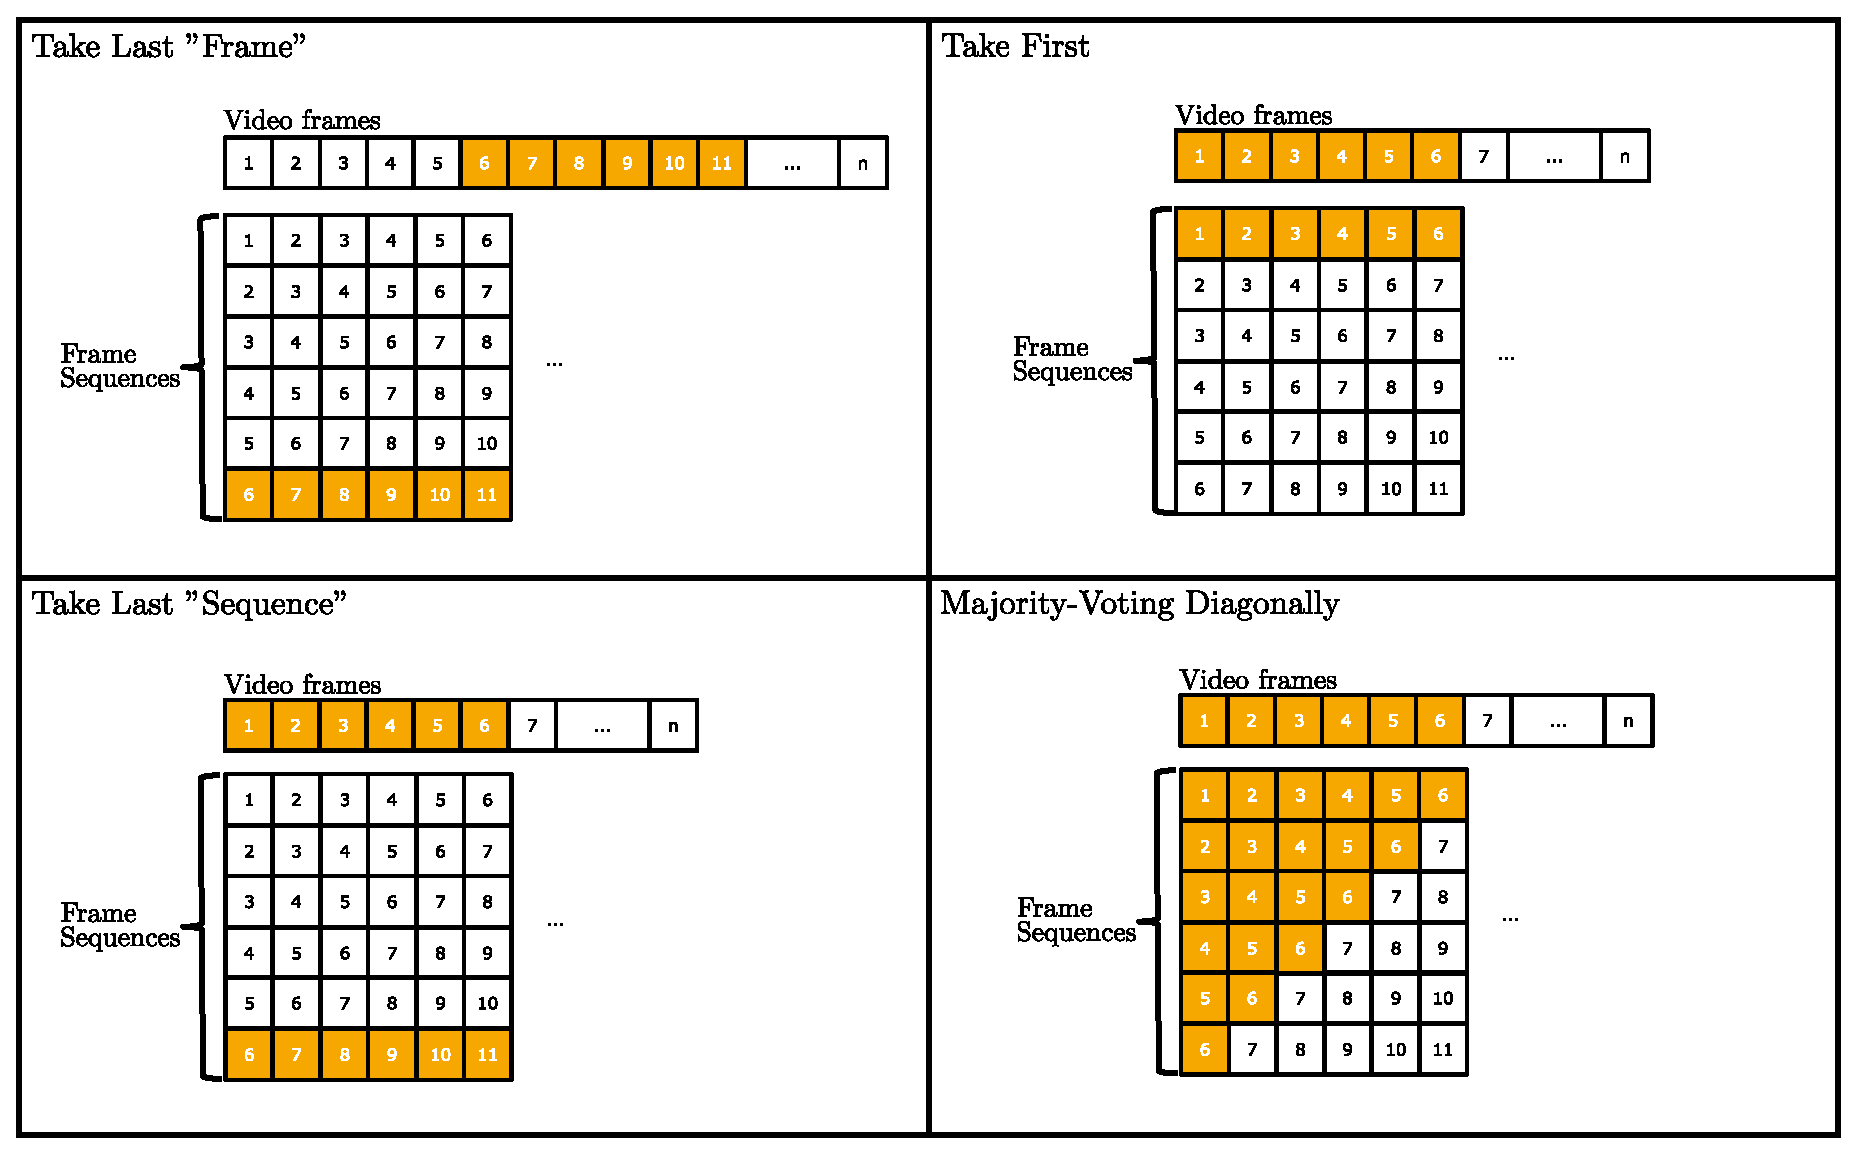
\includegraphics[scale=.5]{images/merging_strategies.eps}
	\caption{To merge the multiple predictions per frame into one, we implemented serval strategies: \textit{Take Last 'Frame'} (top left): The prediction of the frame, where the frame is the last of a frame sequence, is taken. \textit{Take Last 'Sequence'} (bottom left): The last prediction of the frame sequence belonging to a frame is taken. \textit{Take First} (top right): The first prediction of the frame sequence is taken. \textit{Majority-Voting Diagonally} (bottom right): The majority voting among all preditions of the frame is taken.}
	\label{fig:merging_strategies}
\end{figure}
\paragraph{Take First}
A first simple strategy is having a frame, take the first prediction of the frame sequence, belonging to that frame.

\paragraph{Take Last 'Sequence'}
A second simple strategy is having a frame, take the last prediction of a frame sequence, belonging to that frame.
The intuition behind this is, that an RNN/LSTM becomes more and more certain after having seen multiple frames of the sequence.

\paragraph{Take Last 'Frame'}
In the \textit{Take Last 'Frame'} strategy, for every frame the frame sequence, where the frame is the last, is  found. The last prediction in this frame sequence is then taken as prediction for the frame.

\paragraph{Majority-Voting Diagonally}
Each frame is predicted up to \textit{x} times.
In our example it is up to six times.
In the \textit{Majority-Voting Diagonally} all of those predictions are taken and the majority voting among those is taken as prediction for the frame. \\

After merging we have one prediction per frame indicating whether the frame is part of a soft cut or not.
A sequence of frames, which are part of a soft cut, then represent a soft cut.
However, there could be misclassified frame predictions.
We implemented a \textit{Gap Filler} to find and correct some of those misclassified frame predictions.
The \textit{Gap Filler} is looking for sequences of frames, belonging to a soft cut, which are interrupted by some frames, which do not belong to a soft cut.
If the number of interrupting frames is not to large, they will be also classified as soft cut frames.
The idea behind the \textit{Gap Filler} is, that two soft cuts do not occure close to each other.
So, if two soft cuts are only a few frames apart, they probably belong to the same soft cut.
In Figure~\ref{fig:gap_filler} an example of the \textit{Gap Filler} is shown.
Here, a sequence of soft cut frames is interrupted by two non soft cut frames.
Those non soft cut frames are detected by the \textit{Gap Filler} and classified as soft cut frames.
\begin{figure}[!htb]
	\centering
	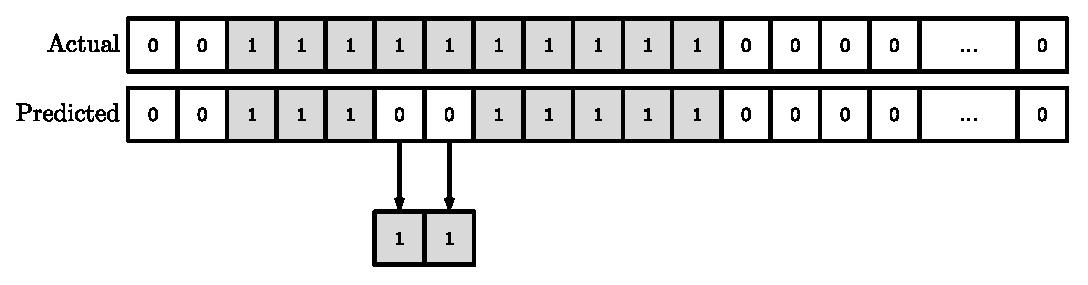
\includegraphics[scale=.7]{images/gap_filler.eps}
	\caption{Two soft cuts do not occure close to each other. Therefore the \textit{Gap Filler} find misclassified frame predictions after the merging step and correct non soft cut frame predictions, if they are interrupting a soft cut.}
	\label{fig:gap_filler}
\end{figure}

Another idea to correct misclassified frame predicitons is to delete soft cuts, which are only up to five frames long and only surrounded by non soft cut frames.
In our data set a soft cut has on average 22 frames.
The smallest have a length of seven frames.
Therefore, a soft cut of only up to five frames is not realistic and misclassified with a high probability.

To classify the frames as soft cut or non soft cut frames, we used an RNN/LSTM.
We tried different architectures, which will be evaluated in Section~\ref{sec:soft_cut_evaluation}.

\paragraph{CNN + one LSTM}
For the CNN we used the architecture of the \textit{caffenet} [TODO: reference].
We also used the pretrained weights of this net, so that we do not need to train our model from sratch.
We only fine-tuned the \textit{fc6} layer of the \textit{caffenet} with a learning rate of 0.1.
The CNN is followed by one LSTM, which weights were initialized with the \textit{Xavier} method [TODO: \url{http://jmlr.org/proceedings/papers/v9/glorot10a/glorot10a.pdf}].
Besides, the general learning rate was set to 0.01 and gradient clipping was used.

\paragraph{CNN + two LSTMs}
The architecture of this net is basically the same as the previous.
There is only one difference: Instead of using just one LSTM, two LSTMs were used.
Also the general learning rate was set to 0.001 and no grandient clipping was used.
The architecture of the net can be found in Figure~\ref{fig:net_architecture}
\begin{figure}[!htb]
	\centering
	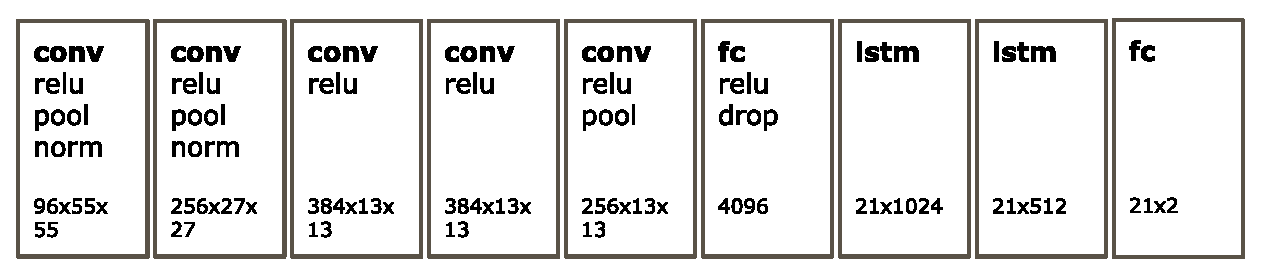
\includegraphics[scale=.5]{images/net_architecture.eps}
	\caption{Architecture of the RNN/LSTM consisting of a CNN and two LSTMs.}
	\label{fig:net_architecture}
\end{figure}

\paragraph{One convolutional layer + two LSTMs}
The last architecture which was tested uses only one convolutional layer before the two LSTMs.
The intuition behind it [TODO].
The net was trained from scratch as no pretrained net existed.
The weights of the LSTMs were again initialized using the \textit{Xavier} method.
The learning rate was 0.001 and gradient clipping was used druing training.